\subsection{SGX Memory Access Protection}
\label{sec:sgx_access_protection}

SGX guarantees that the software inside an enclave is isolated from all the
software outside the enclave, including the software running in other enclaves.
This isolation guarantee is at the core of SGX's security model.

It is tempting to assume that the main protection mechanism in SGX is the
Memory Encryption Engine (MEE) described in
\S~\ref{sec:sgx_uncore_modifications}, as it encrypts and MACs the DRAM's
contents. However, the MEE sits in the processor's memory controller, which is
at the edge of the on-chip memory hierarchy, below the
caches~(\S~\ref{sec:caching}). Therefore, the MEE cannot protect an enclave's
memory from software attacks.

% Page-Based Access Control: SDM S 38.5
% Interactions with Paging: SDM S 42.4
% ISCA SGX Slide 27

The root of SGX's protections against software attacks is a series of memory
access checks which prevents the currently running software from accessing
memory that does not belong to it. Specifically, non-enclave software is only
allowed to access memory outside the PRM range, while the code inside an
enclave is allowed to access non-PRM memory, and the EPC pages owned by the
enclave.

Although it is believed~\cite{evtyushkin2014isox} that SGX's access checks are
performed on every memory access checks, all our information sources indicate
that the access checks are only performed during TLB misses. The intuition
behind this finding can be built by considering what it would take to implement
SGX's memory access protections in a trusted operating system or hypervisor,
solely by using the page tables that direct the CPU's address
translation feature~(\S~\ref{sec:paging}).

The hypothetical trusted software described above can implement enclave
entry~(\S~\ref{sec:sgx_eenter}) would be implemented as a system
call~\S~\ref{sec:syscalls} that creates page table entries mapping the
enclave's memory. Enclave exit~(\S~\ref{sec:sgx_eexit}) can be a symmetric
system call that removes the page table entries created during enclave entry.
When modifying the page tables, the system software has to consider TLB
coherence issues~(\S~\ref{sec:tlbs}) and perform TLB shootdowns when
appropriate.

% Enclave Page Cache Map (EPCM): SDM S 37.5.1, SDM S 38.19
% SECINFO.FLAGS: SDM S 38.11.1
% PAGE_TYPE Field Definition: SDM S 38.11.2

SGX leaves page table management under the system software's control, but it
cannot trust the software to set up the page tables in any particular way.
Therefore, the hypothetical design described above cannot be used by SGX as-is.
Instead, at a conceptual level, the SGX implementation approximates the effect
of having the page tables set up correctly by inspecting every address
translation that comes out of the Page Miss Handler~(PMH,~\S~\ref{sec:tlbs}).
The address translations that do not obey SGX's access control restrictions
are rejected before they have a chance to reach the TLBs and be used to service
load and store instructions.

When an address translation (\S~\ref{sec:paging}) result is the physical
address of an EPC page, the CPU ensures\footnote{A mismatch triggers a general
protection fault (\#GP, \S~\ref{sec:faults}).} that the virtual address given
to the address translation process matches the expected virtual address
recorded in the page's EPCM entry, as shown in
Figure~\ref{fig:sgx_tlb_miss_checks}. This prevents the system software, which
manages the page tables and EPT, from modifying an enclave's virtual address
space in a manner that is inconsistent with the enclave author's expectations.

\begin{figure}[hbt]
  \centering
  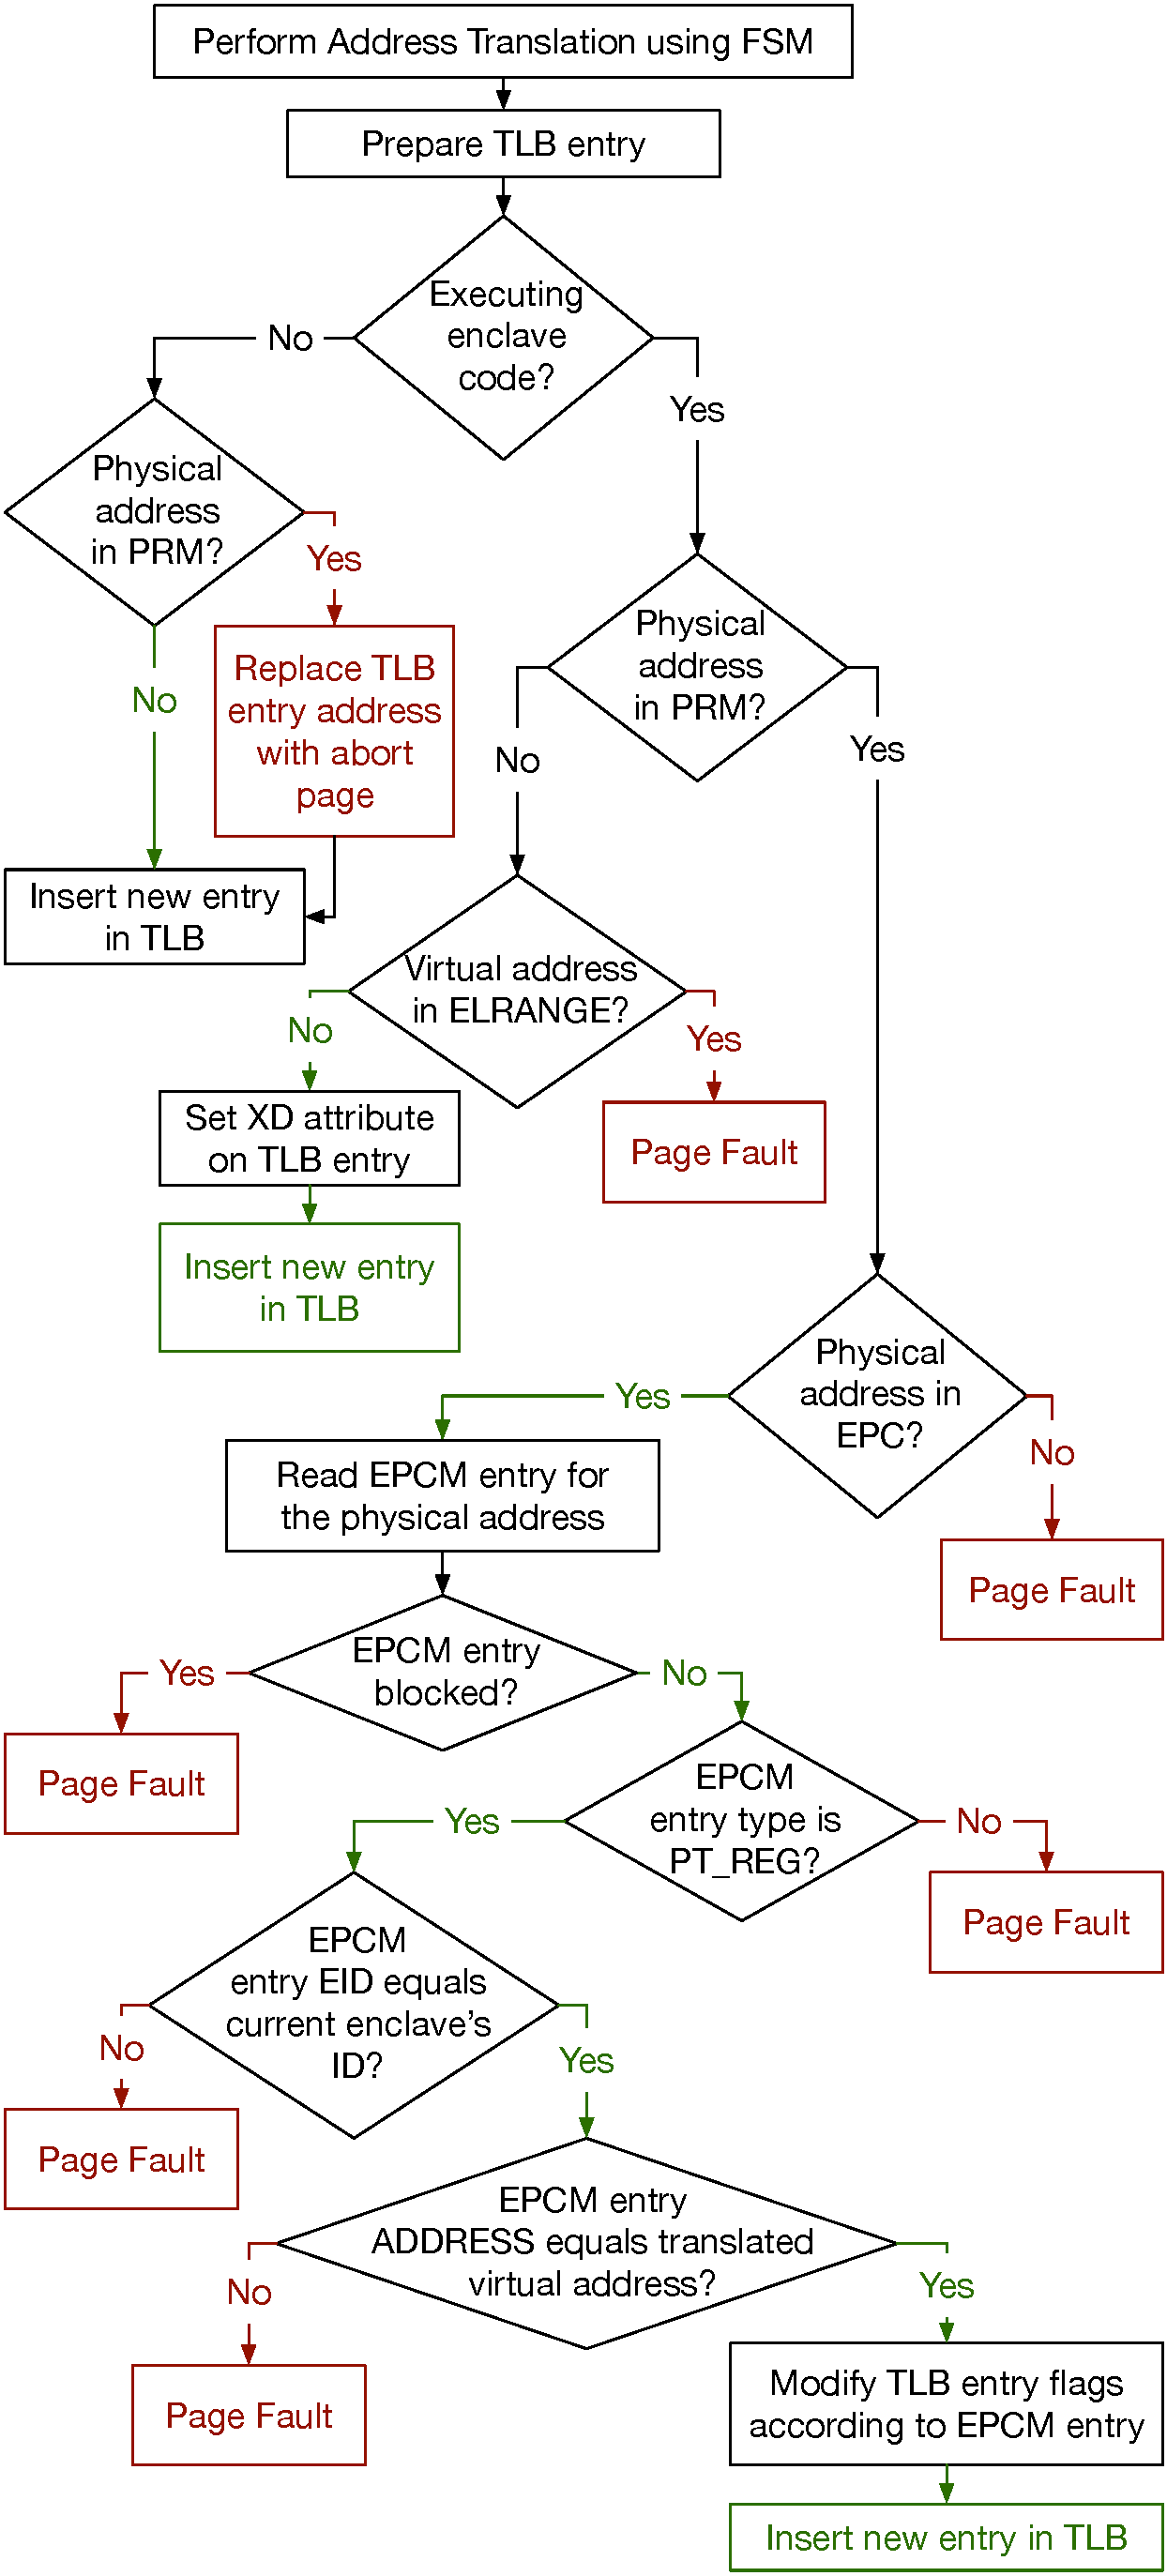
\includegraphics[width=85mm]{figures/sgx_tlb_miss_checks.pdf}
  \caption{
    The access control logic added by SGX to the PMH
  }
  \label{fig:sgx_tlb_miss_checks}
\end{figure}

SGX's security revolves around maintaining the following
invariant. \textbf{At all times, a logical processor's TLB
entries can only map DRAM pages that can be accessed by the code executing on
the processor.} Specifically, when a logical processor is in enclave mode, its
TLB can include entries for the enclave's EPC pages, and for DRAM pages outside
the PRM. The TLB of a logical processor outside enclave mode must not include
any PRM entry.

Without any special measures, the invariant described above would be broken
when a logical processor exits an enclave, either via
\texttt{EEXIT}~(\S~\ref{sec:sgx_eexit}), or via an AEX~(\S~\ref{sec:sgx_aex}).
This is because enclave mode allows TLB entries that point to the currently
executing enclave's EPC pages, and these entries become disallowed the moment
the processor leaves enclave mode. The SGX implementation solves this problem
by flushing a logical processor's TLBs when it leaves enclave mode.
